\documentclass[tikz]{standalone}

\usepackage[greek,english]{babel}

\usepackage{pgfplots}
\usetikzlibrary{decorations.pathreplacing}

\pagecolor{white}

\begin{document}
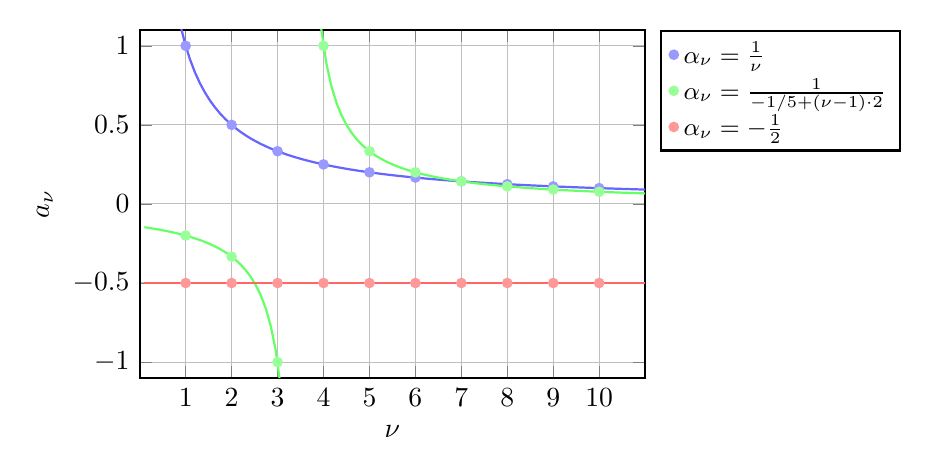
\begin{tikzpicture}
\begin{axis}[
    width=8cm,
    height=6cm,
    domain=-15:15, 
    restrict y to domain=-50:50,
    xmin=0,
    xmax=11,
    ymin=-1.1,
    ymax=1.1,
    ytick={-1,-0.5, 0,0.5,1},
    thick,
    xtick=data,
    legend pos=outer north east,
    mark size=1.5pt,
    xlabel={$\nu$},
    ylabel={$a_\nu$},
    legend cell align={left},
    grid]


\addplot[only marks, blue!40!white] coordinates {
(1, 1)
(2, 0.5)
(3, 0.333333)
(4, 0.25)
(5, 0.2)
(6, 0.166667)
(7, 0.142857)
(8, 0.125)
(9, 0.111111)
(10, 0.1)
};
\addlegendentry{\small $\alpha_\nu = \frac{1}{\nu}$ }

\addplot[red, domain=0.1:11,restrict y to domain=0:18, samples=100, blue!60!white,forget plot]  {1/x};


\addplot[only marks, green!40!white] coordinates {
(1, -0.2)
(2, -0.333333)
(3, -1)
(4, 1)
(5, 0.333333)
(6, 0.2)
(7, 0.142857)
(8, 0.111111)
(9, 0.0909091)
(10, 0.0769231)
};
\addlegendentry{\small $\alpha_\nu = \frac{1}{-1/5 + (\nu - 1) \cdot 2}$ }

\addplot[domain=0.1:11,restrict y to domain=-18:18, samples=100, green!60!white,forget plot]  {1/(-5 + (x-1)*2)};

\addplot[only marks, red!40!white] coordinates {
(1, -0.5)
(2, -0.5)
(3, -0.5)
(4, -0.5)
(5, -0.5)
(6, -0.5)
(7, -0.5)
(8, -0.5)
(9, -0.5)
(10, -0.5)
};
\addlegendentry{\small $\alpha_\nu = -\frac{1}{2}$ }

\addplot[domain=0.1:11,restrict y to domain=-1:18, samples=100, red!60!white,forget plot]  {-0.5};

\end{axis}
\end{tikzpicture}
\end{document}
